\subsection{Theorem}
\begin{namedframe}{Theorem}
	\begin{theorem}[``Crossed Chord'' Theorem]
		If two chords $AB$ and $CD$ of a circle intersect at point $P$, then $(PA)(PB) = (PC)(PD)$.
	\end{theorem}
	\vspace{-2ex}
	\begin{center}
		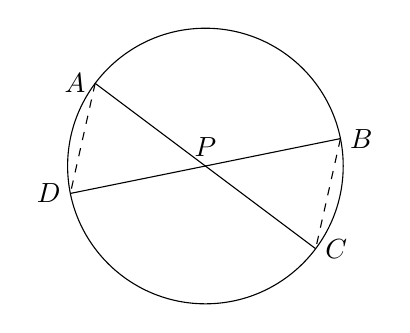
\begin{tikzpicture}[scale=0.35]
			\coordinate [label=above:$P$](P) at (0,0);
			\coordinate [label=left:$A$](A) at (-4,3);
			\coordinate [label=right:$B$](B) at (4.9,0.994987437107);
			\coordinate [label=right:$C$](C) at (4,-3);
			\coordinate [label=left:$D$](D) at (-4.9,-0.994987437107);

			\draw (P) circle (5);
			\draw (A) -- (P) -- (B);
			\draw (D) -- (P) -- (C);
			\draw [dashed] (B) -- (C);
			\draw [dashed] (A) -- (D);
		\end{tikzpicture}
	\end{center}
	\vsep[-2ex]
	This is proved using similar triangles and the fifth extension we developed for the Star Trek theorem.
	Try to prove it yourself!
\end{namedframe}
